% FAA-Net Architecture Diagram using TikZ
% Compile with pdflatex or include in your main document
% Required packages: tikz, positioning, shapes, arrows

\documentclass[border=10pt]{standalone}
% If including in main document, remove the documentclass and standalone package

\usepackage{tikz}
\usetikzlibrary{positioning, shapes.geometric, arrows.meta, calc, fit, backgrounds}

% Define custom colors
\definecolor{novelcolor}{RGB}{255,165,0}      % Orange for novel contribution
\definecolor{inputcolor}{RGB}{173,216,230}    % Light blue for input/output
\definecolor{standardcolor}{RGB}{220,220,220} % Light gray for standard components

% Define styles
\tikzset{
    block/.style={
        rectangle, rounded corners,
        draw, thick,
        minimum height=1.2cm,
        text centered,
        font=\small
    },
    novelblock/.style={
        block,
        fill=novelcolor!30,
        draw=novelcolor!80,
        minimum width=3.5cm
    },
    inputblock/.style={
        block,
        fill=inputcolor!40,
        draw=inputcolor!80,
        minimum width=2cm
    },
    standardblock/.style={
        block,
        fill=standardcolor!40,
        draw=gray!80,
        minimum width=2.2cm
    },
    smallblock/.style={
        block,
        fill=standardcolor!30,
        draw=gray!60,
        minimum width=1.8cm,
        minimum height=0.8cm,
        font=\footnotesize
    },
    arrow/.style={
        -Stealth,
        thick
    },
    dottedarrow/.style={
        -Stealth,
        thick,
        dotted
    },
    label/.style={
        font=\tiny,
        text=gray
    }
}

\begin{document}

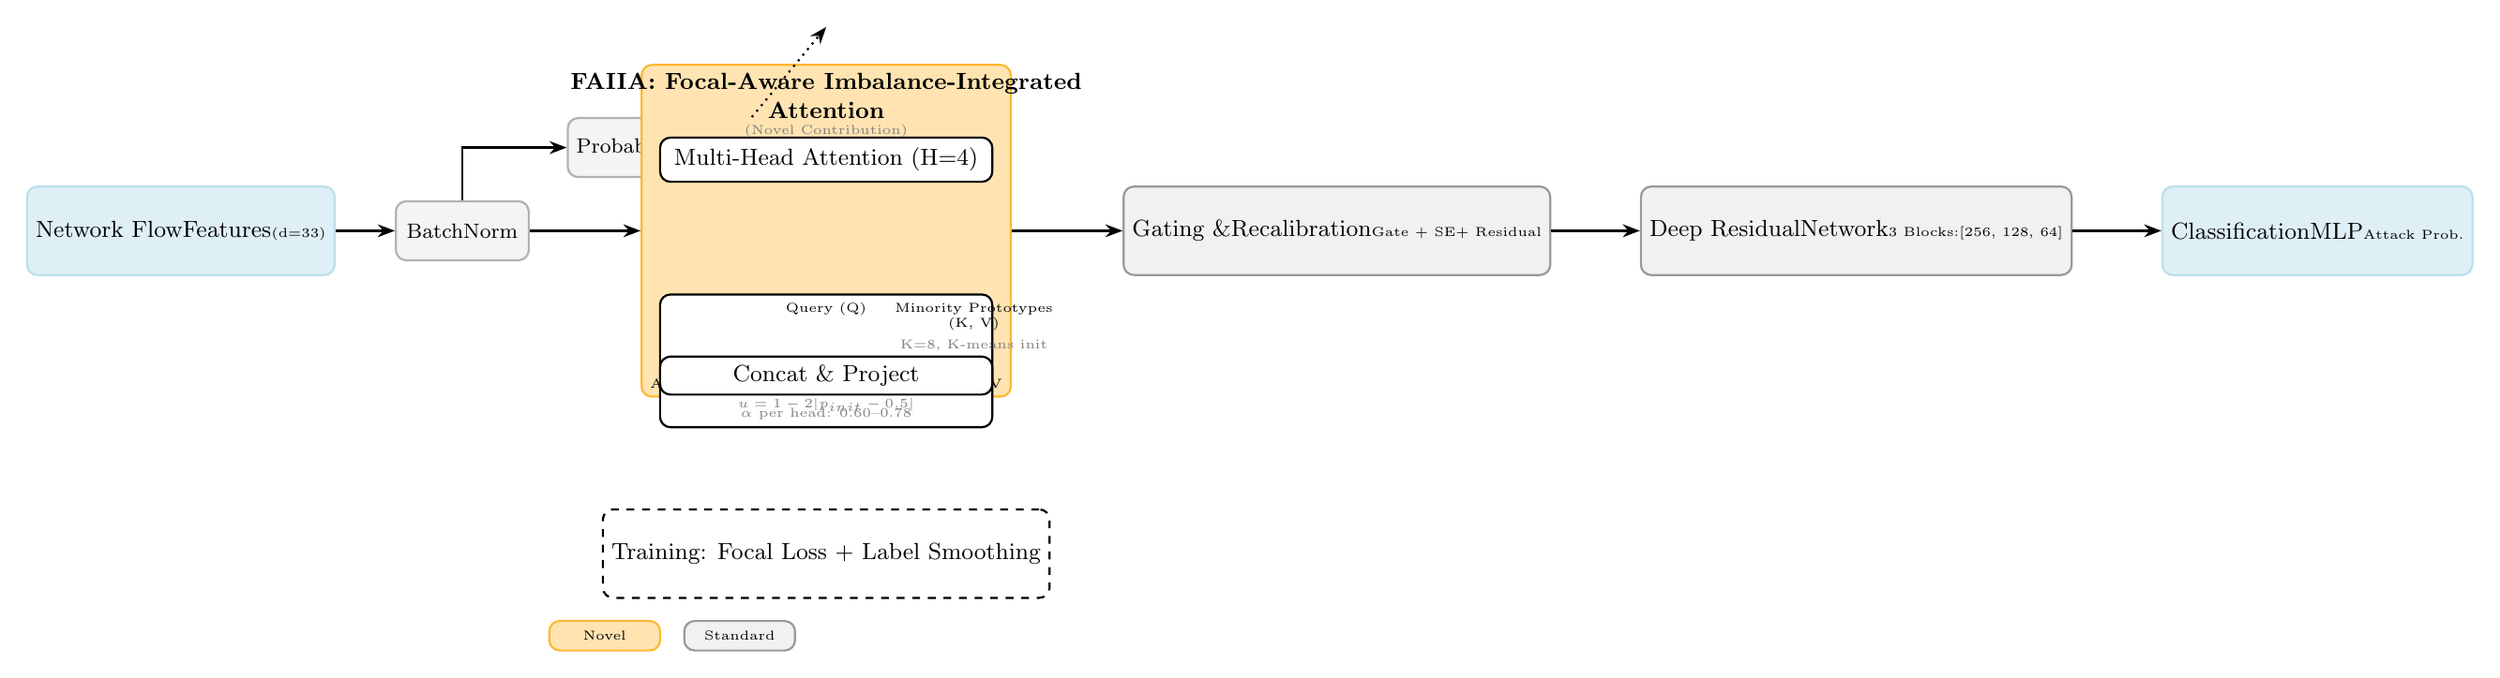
\begin{tikzpicture}[node distance=1.5cm and 1.2cm]

% Input
\node[inputblock] (input) {Network Flow\\Features\\{\tiny (d=33)}};

% Batch Norm
\node[smallblock, right=0.8cm of input] (bn) {Batch\\Norm};

% Probability Estimator (top path)
\node[smallblock, above right=0.3cm and 0.5cm of bn] (prob) {Probability\\Estimator\\{\tiny 2-layer MLP}};
\node[label, below=0.1cm of prob] (pinit) {$p_{\text{init}}$};

% FAIIA Module (main component)
\node[novelblock, right=1.5cm of bn, minimum width=5cm, minimum height=4.5cm] (faiia) {};

% FAIIA Title
\node[anchor=north, font=\bfseries\small] at (faiia.north) {FAIIA: Focal-Aware Imbalance-Integrated};
\node[anchor=north, font=\bfseries\small] at ([yshift=-0.4cm]faiia.north) {Attention};
\node[anchor=north, font=\tiny, text=gray] at ([yshift=-0.7cm]faiia.north) {(Novel Contribution)};

% FAIIA Internal components
\node[block, fill=white, minimum width=4.5cm, minimum height=0.6cm] at ([yshift=-1.3cm]faiia.north) (multihead) {Multi-Head Attention (H=4)};

% Attention mechanism box
\node[block, fill=white, minimum width=4.5cm, minimum height=1.8cm] at ([yshift=0.5cm]faiia.south) (attn) {};
\node[font=\tiny] at ([yshift=0.7cm]attn.center) {Query (Q)};
\node[font=\tiny] at ([yshift=0.7cm, xshift=2cm]attn.center) {Minority Prototypes};
\node[font=\tiny] at ([yshift=0.5cm, xshift=2cm]attn.center) {(K, V)};
\node[font=\tiny, text=gray] at ([yshift=0.2cm, xshift=2cm]attn.center) {K=8, K-means init};
\node[font=\tiny, align=center] at ([yshift=-0.3cm]attn.center) {Attention = softmax$((1 + \alpha \cdot u^\gamma) \cdot$ Q·K$^T) \cdot$ V};
\node[font=\tiny, text=gray] at ([yshift=-0.6cm]attn.center) {$u = 1-2|p_{\text{init}}-0.5|$};

% Concat & Project
\node[block, fill=white, minimum width=4.5cm, minimum height=0.5cm] at ([yshift=0.3cm]faiia.south) (concat) {Concat \& Project};
\node[label, below=0.05cm of concat] {$\alpha$ per head: 0.60--0.78};

% Post-processing
\node[standardblock, right=1.5cm of faiia] (gating) {Gating \&\\Recalibration\\{\tiny Gate + SE}\\{\tiny + Residual}};

% Feature Extraction
\node[standardblock, right=1.2cm of gating] (resnet) {Deep Residual\\Network\\{\tiny 3 Blocks:}\\{\tiny [256, 128, 64]}};

% Classification
\node[inputblock, right=1.2cm of resnet] (classifier) {Classification\\MLP\\{\tiny Attack Prob.}};

% Training (bottom)
\node[block, dashed, fill=white, below=1.5cm of faiia, minimum width=6cm] (loss) {Training: Focal Loss + Label Smoothing};

% Arrows - Main flow
\draw[arrow] (input) -- (bn);
\draw[arrow] (bn) -- (faiia);
\draw[arrow] (faiia) -- (gating);
\draw[arrow] (gating) -- (resnet);
\draw[arrow] (resnet) -- (classifier);

% Arrows - Probability estimator
\draw[arrow] (bn) |- (prob);
\draw[dottedarrow] (prob) -- ([yshift=0.5cm]faiia.north);

% Legend
\node[novelblock, minimum width=1.5cm, minimum height=0.4cm, font=\tiny] at ([xshift=-3cm, yshift=-0.5cm]loss.south) (leg1) {Novel};
\node[standardblock, right=0.3cm of leg1, minimum width=1.5cm, minimum height=0.4cm, font=\tiny] (leg2) {Standard};

\end{tikzpicture}

\end{document}
